\chapter{Conclusion}\label{ch:conclusion}
\setlength{\epigraphwidth}{0.90\textwidth}
\epigraph{``We are all shaped by the tools we use, in particular: the formalisms we use shape our thinking habits, for better or for worse, and that means that we have to be very careful in the choice of what we learn and teach, for unlearning is not really possible.''}{\begin{flushright}--Edsger W. \citet{dijkstra2000answers}, \href{https://www.cs.utexas.edu/~EWD/transcriptions/EWD13xx/EWD1305.html}{\textit{Answers to questions from students of Software Engineering}}\end{flushright}}

In this thesis, we explored four different programming tools from software engineering for the development of intelligent systems, broadly addressing cognitive complexity arising in four phases of Royce's Waterfall method (\autoref{fig:waterfall_model}). These tools have varying degrees of practicality, from highly theoretical (e.g. adversarial testing of differentiable programs ~\autoref{ch:difftest}) to more pragmatic (e.g. containerization ~\autoref{ch:ducker}). In each chapter, we provide some motivating examples which demonstrate key deficiencies in state-of-the-art programming tools for intelligent systems and propose viable solutions which address a few of those shortcomings. While we hope that intelligent system programmers (e.g. roboticists and machine learning practitioners) may derive some value from the tools themselves, our intention is to be \textit{illustrative} rather than \textit{prescriptive}.

In building tools and validating their effectiveness on toy applications, it is our hope that tool developers will carefully consider how software tools can introduce and mitigate cognitive complexity. Well designed tools can augment the cognitive capacity of humans to reason about facts in the presence of uncertainty~\citep{famelis2012partial}, and provide ergonomic debugging and visualization assistance (e.g. \autoref{ch:hatchery}). We also hope to convey the importance of notational design. Good notation forces authors to think carefully about their abstractions, makes logical errors conspicuous, and helps them to understand the implications of early design choices. We hope that the programming tools presented in this thesis will inspire developers to re-imagine the potential for computer-aided programming in designing software for intelligent systems.

By complementing the cognitive abilities of human programmers -- who excel at creative problem solving and high-level abstract reasoning -- with the raw symbolic processing abilities of programming tools, we can accelerate the design~\autoref{ch:hatchery}, development~\autoref{ch:kotlingrad}, validation~\autoref{ch:difftest} and deployment~\autoref{ch:ducker} of intelligent systems in real-world applications. This process is a virtuous cycle which deserves domain-specific tools and practices due to the opportunities which intelligent systems afford and the unique interplay between human and machine intelligence. As we begin to develop autonomous systems which play increasingly active roles in society, both software engineers and machine learning practitioners must play a similarly active role in shaping the behavior of those systems.

Software engineers have a number of lessons to learn from intelligent systems. Language designers would do well to consider the value of smart developer tools (\autoref{ch:hatchery}) in facilitating the dialogue between human and machine intelligence. Languages should strive to incorporate human knowledge via differentiable programming and expert systems, to help reason about compositionality and denotational correctness (\autoref{ch:kotlingrad}). Automated testing via simulators and property testing frameworks is needed to reason about operational correctness without exhaustive specification (\autoref{ch:difftest}). Finally, continuous integration, automated testing and best practices in developer operations (\autoref{ch:ducker}) are needed to ensure reproducible artifacts in the presence of software and hardware variability.

Machine learning practitioners also have a number of lessons to learn from software engineering. Traditional software engineering prescribes a rigorous process model and testing methodology (\autoref{fig:waterfall_model}) which has guided many generations of software projects. To become a true engineering discipline, machine learning will need a more systematic approach to building autonomous systems. Machine learning models are trained on \textit{objective functions}, which are typically low-dimensional functions measuring the performance of a system, returning a scalar value known as an \textit{error} or \textit{loss}. In practice, intelligent systems must satisfy a multiobjective set of criteria~\citep{censi2015mathematical}, including energy efficiency~\citep{paull2010novel}, memory~\citep{memory2013mitliagkas}, re/usability~\citep{breuleux2017automatic,deleu2019torchmeta}, predictability~\citep{turner2017well}, latency~\citep{ravanelli2018twin}, robustness~\citep{pineau2003policy}, reproducibility~\citep{pineau2019improving}, explainability~\citep{turner2016model}, traceability~\citep{guo2017semantically, tsirigotis2018orion}, uncertainty~\citep{diaz2018interactive}, simplicity~\citep{kastner2019representation}, trustworthiness~\citep{xu2017efficient}, transferability~\citep{mehta2019active}, scalability~\citep{luan2019break} and many other factors.

In traditional software engineering, it is reasonable to assume those implementing a new system have some implicit domain knowledge and are well-intentioned human beings working towards a common goal. Given a coarse description, they can fill in the blanks. When building an intelligent system, we would be safer to assume the requirements are implemented by a genie. Given some data and an optimization metric, it will take every available shortcut to grant our wishes. If we are not careful about stating our requirements, this entity will produce a solution that simply does not work (in the best case), or appears to work but is truly cursed~\citep{bellman1957dynamic}.

When building an intelligent system, developers must carefully ask, ``What is the desired behavior of the system we are designing?'' This question is often very troublesome, for our approximate requirements must be translated into precise constraints on the solution space. For example, when designing a self-driving vehicle, we must clearly optimize for passenger safety, however doing so na\"ively will train a vehicle that never moves, or always yields to passing vehicles. Short of exhaustive specification, how can we be assured the resulting system satisfies our requirements? Most humans are capable of safely driving a vehicle, but even the best engineers are hard-pressed when asked to write a driving algorithm. Labeling the data by hand is too expensive. Formal verification is right out the window.

\begin{figure}
    \centering
    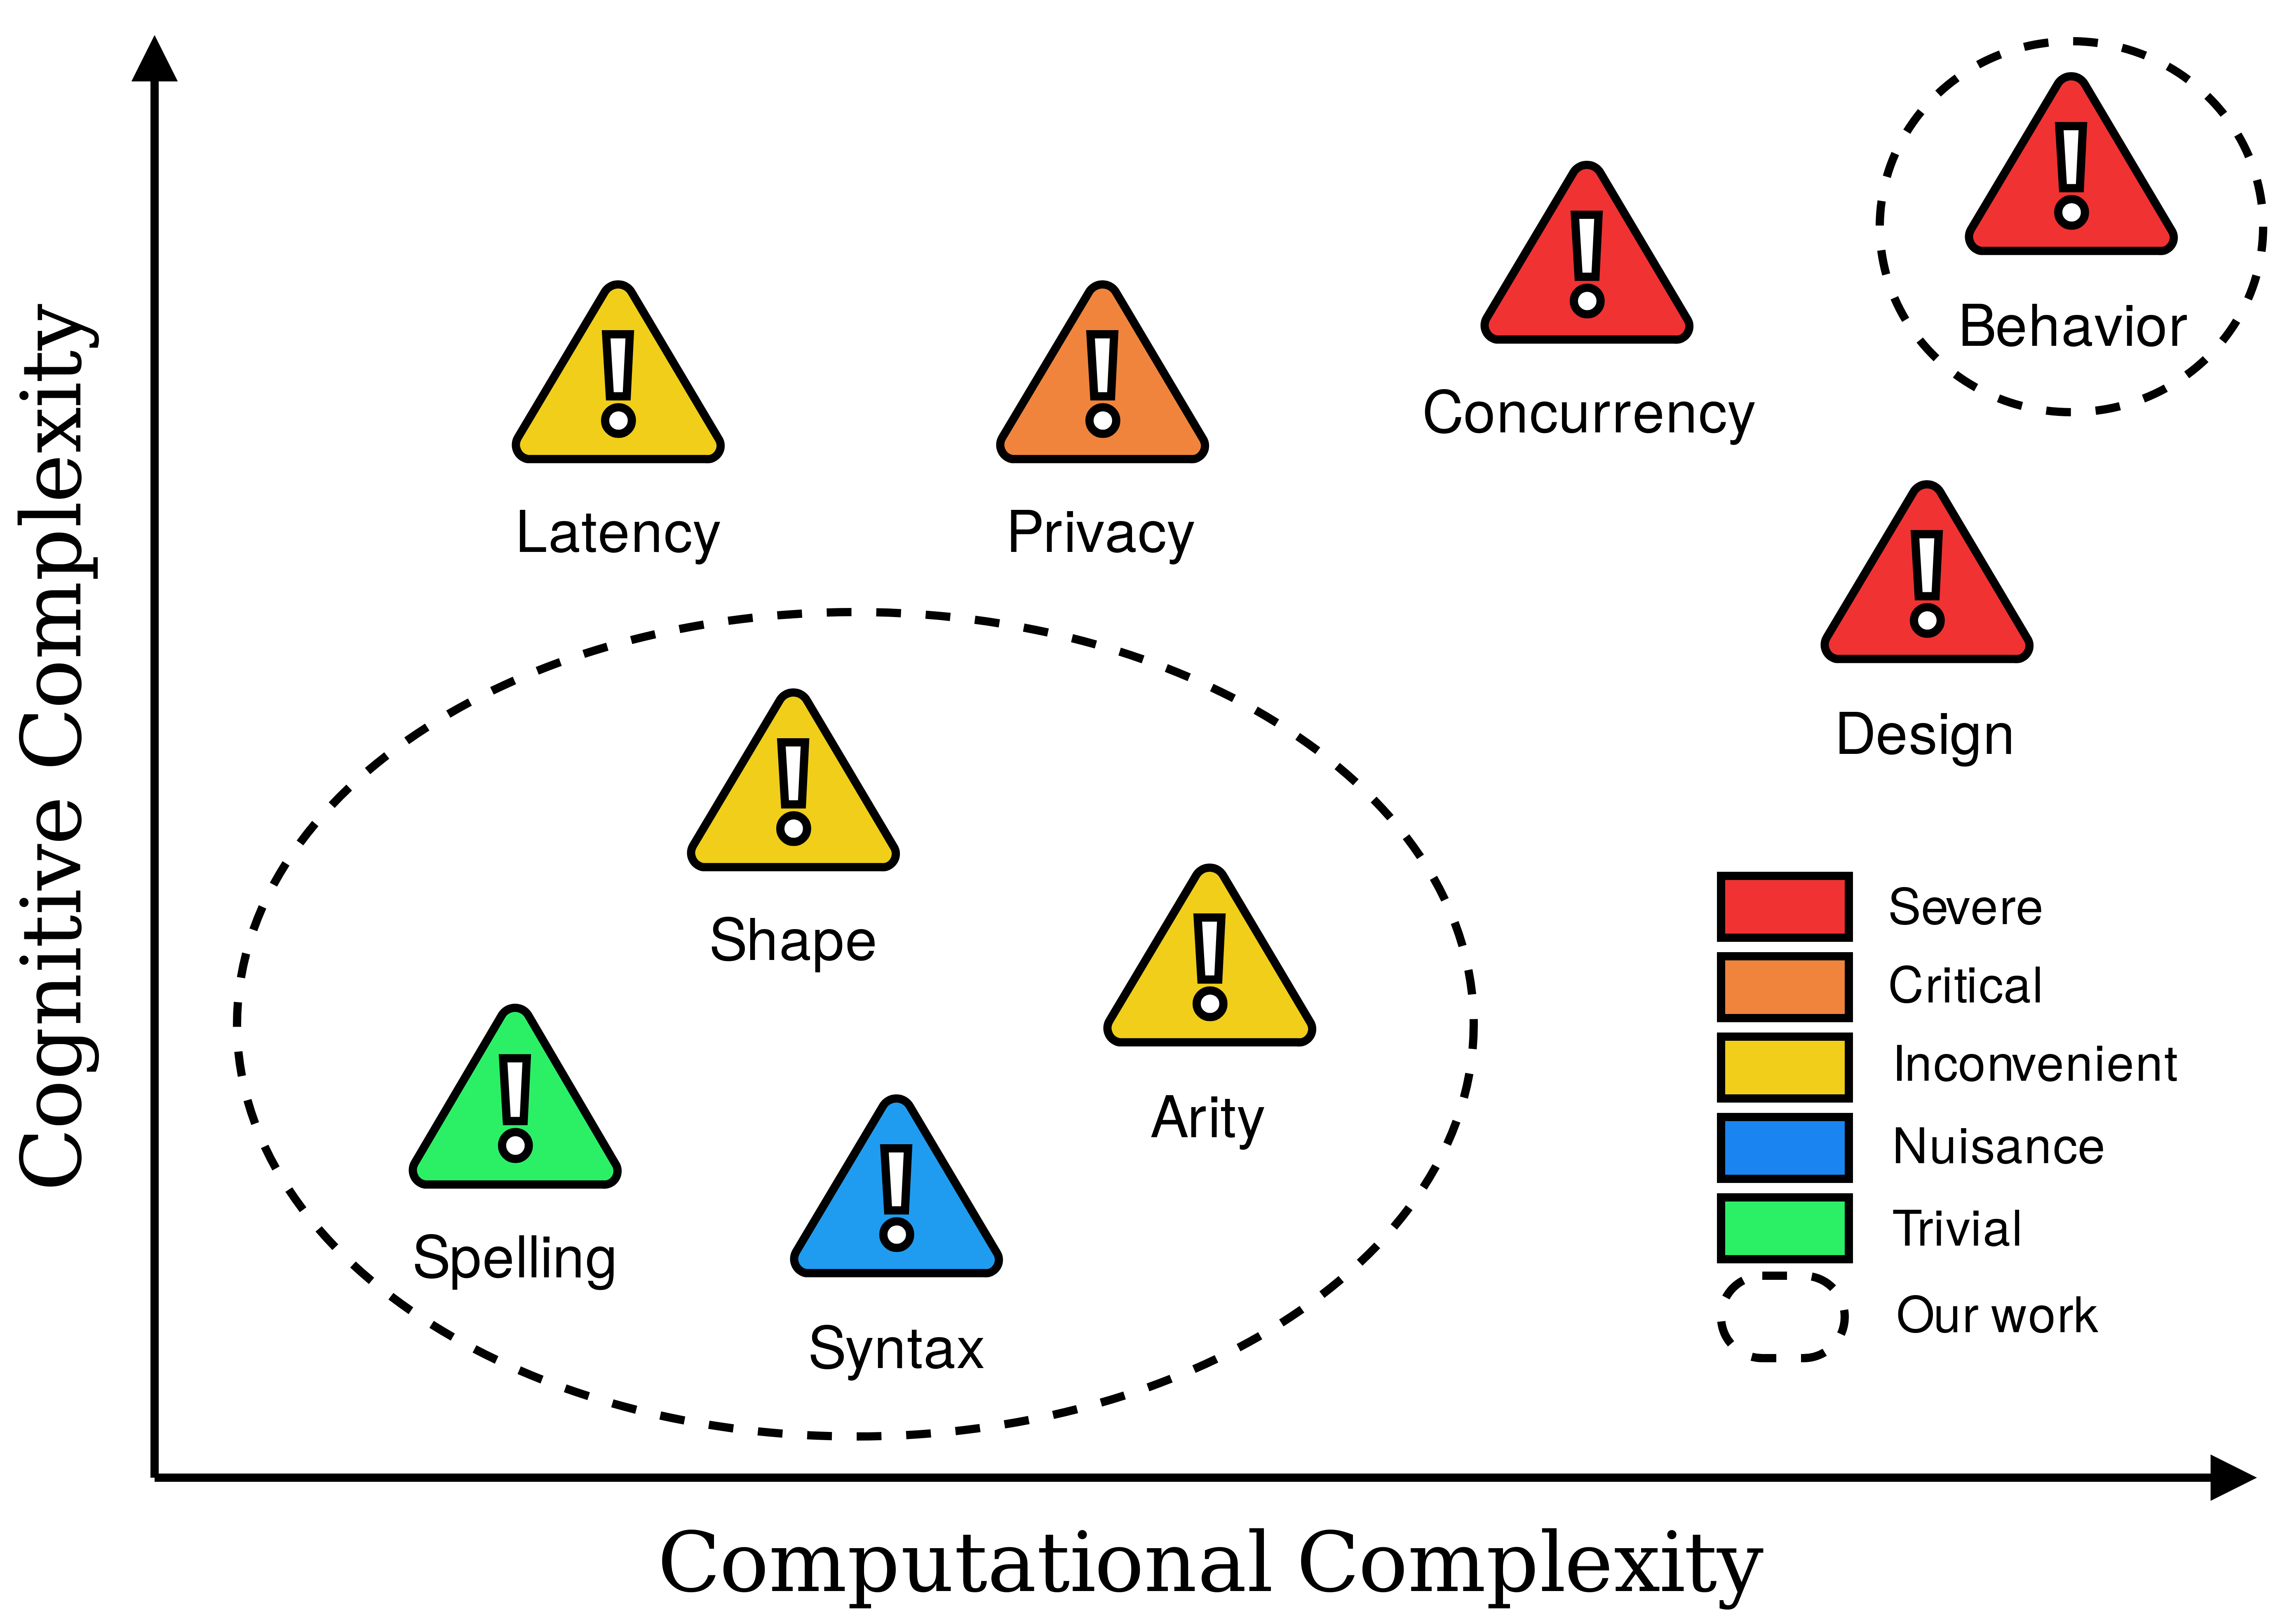
\includegraphics[width=0.60\textwidth]{../figures/verification_complexity.png}
    \caption{Complexity of detecting various types of programming errors.}
    \label{fig:verification_complexity}
\end{figure}

Type systems, compilers and fuzzers are all part of a broader class of validation and verification tools. The goal of these tools is to trade cognitive complexity for computational complexity. Some errors (e.g. syntactical errors), are minor nuisances and can be detected with a good incremental parser (\autoref{subsec:the-parser}). Others, as shown in~\autoref{fig:verification_complexity}, have higher cognitive complexity but can be detected by spending computation. We argue this computational cost is often justified as computation is cheap and bugs can have catastrophic consequences. Studies show the earlier bugs are detected, the more likely they are to be fixed~\citep{distefano2019scaling} -- saving minutes in development could save lives during operation. Spending computation also frees up valuable cognitive resources for other tasks.

Fuzz testing remains an economically and computationally efficient alternative to formal verification. As shown in \autoref{sec:prob_ad_test}, we can detect more severe errors with a lower fiscal and computational budget by making some practical assumptions about the model and oracle. As today's engineers begin to add learning capabilities to tomorrow's safety-critical robotic systems, we believe the increased assurance intelligent validation and verification tools provide will be indispensable for scaling up these complex adaptive cyberphysical systems.

Much work remains for the interested reader. A great deal of work in machine learning is designing representations which are suitable for downstream tasks and loss functions which accurately measure performance on those tasks. Building representations and loss functions which capture the full range of objectives can be a painstaking process to debug. We encourage engineers to think carefully the process of debugging machine learning models and how we can accelerate the lifecycle, from data mining and analysis to evaluation and deployment.

Machine learning researchers would do well to consider the value of denotational semantics for grounding and reasoning about specifications. While type-theoretic verification tools are currently limited to simple properties, their abstractions are very powerful. Whether type systems or expert systems, computer aided reasoning tools will play an important role in the development of safe intelligent systems. We encourage the reader to look carefully at the value these systems provide, and when they are unsuitable, consider using property checking techniques and continuous integration methods for ensuring functional correctness.

\section{Contributions}

There are many interesting codesign problems at the intersection of tools, languages and systems (\autoref{fig:venn_triagram}). In this work, we consider the theory and implementation of programming tools for intelligent systems. The opposite direction is also an intriguing subject, but remains outside the scope of this thesis. Language designers have recently begun to explore the meaning of ``toolable'' languages and tooling-enhanced languages~\citep{chatley2019next}. Research in language oriented programming~\citep{dmitriev2004language} and model-driven engineering~\citep{famelis2015mummint} has also considered tools for API and PL designers. Software engineers have studied a number of tools for intelligent systems including notebooks~\citep{chattopadhyays2020notebooks}, REPLs and interactive programming environments. Finally, languages and intelligent systems have enjoyed a fruitful collaboration in differentiable and probabilistic programming (\autoref{sec:differentiable-programming}). Each of these would be an interesting thesis in its own right.

\begin{figure}

    \begin{tikzpicture}[{every node/.style={black,font=\sffamily\Large}}]
        \def\firstcircle{(0,0) circle (3cm)}
        \def\secondcircle{(3.6,0) circle (3cm)}
        \def\thirdcircle{(1.8,3.6) circle (3cm)}
        \def\boundingbox{(-3,-3) rectangle (6,4.5)}

        \definecolor{handsome}{HTML}{C8CADF}
        \definecolor{jerk}{HTML}{EF3A43}
        \definecolor{batman}{HTML}{FBC405}
        \definecolor{dumb}{HTML}{B7CA54}
        \definecolor{smart}{HTML}{C7DAC4}
        \definecolor{nerd}{HTML}{4C4B6B}
        \definecolor{nice}{HTML}{E4B1AD}

        % fill circles
        \fill[smart] \firstcircle node[xshift=-1.7cm, yshift=-0.3cm, text width=1cm] {Intelligent\\Systems};
        \fill[nice] \secondcircle node[xshift=0.15cm, yshift=-0.3cm, text width=1cm] {Programming\\Languages};
        \fill[handsome] \thirdcircle node[yshift=-0.5cm, yshift=1cm] {Developer Tools};

        \drawcircle
        % fill intersections
        % intersection of first and second
        \begin{scope}
            \clip \boundingbox \thirdcircle;
            \clip \firstcircle;
            \fill[nerd] \secondcircle node[black, xshift=-1.5cm, yshift=-.5cm];
        \end{scope}
        % intersection of first and third
        \begin{scope}
            \clip \boundingbox \secondcircle;
            \clip \firstcircle;
            \fill[jerk] \thirdcircle node[xshift=-1.8cm, yshift=-1cm];
        \end{scope}
        % intersection of second and third
        \begin{scope}
            \clip \boundingbox \firstcircle;
            \clip \secondcircle;
            \fill[dumb] \thirdcircle node[xshift=1.8cm, yshift=-1cm];
        \end{scope}
        % intersection of first, second and third
        \begin{scope}
            \clip \firstcircle;
            \clip \secondcircle;
            \clip \thirdcircle;
            \fill[batman] \boundingbox;
        \end{scope}
        \node at (1.2,1.2)[text width=0.2cm, align=center] {Thesis};
    \end{tikzpicture}
    \caption{Many interesting applications lie at the intersection of these three fields.}
    \label{fig:venn_triagram}
\end{figure}

Our contributions in this particular thesis are fourfold. In \autoref{ch:hatchery}, we introduce a new plugin for the IntelliJ Platform, an integrated development environment with support for the Robot Operating System. In addition to applications-driven frameworks like ROS, several domain specific languages for intelligent systems have recently emerged (\autoref{sec:differentiable-programming}). In \autoref{ch:kotlingrad} we introduce one more, an embedded DSL in the Kotlin language allowing users to write shape-safe differentiable programs in a mathematically idiomatic notation.

Reproducibility is a broad challenge in intelligent systems design, requiring a multi-pronged solution. We believe testing and validation of intelligent systems will play an important role in safety-critical applications. Automated testing and simulation, as well reproducible build and deployment tools will be essential for robustness. In \autoref{ch:difftest}, we introduce a general purpose property-based testing algorithm and empirically show an improvement in data efficiency by detecting a greater proportion of errors in a fixed computational budget. Finally, in \autoref{ch:ducker}, we present a fully-containerized build environment and continuous integration workflow, improving the re/usability and re/producibility of software applications on the Duckietown platform. Together, these contributions help to alleviate cognitive complexity when designing, developing, testing and deploying intelligent systems.